\chapter{Architecture et description de l'application}

\section{Architecture des modules}
\begin{center}
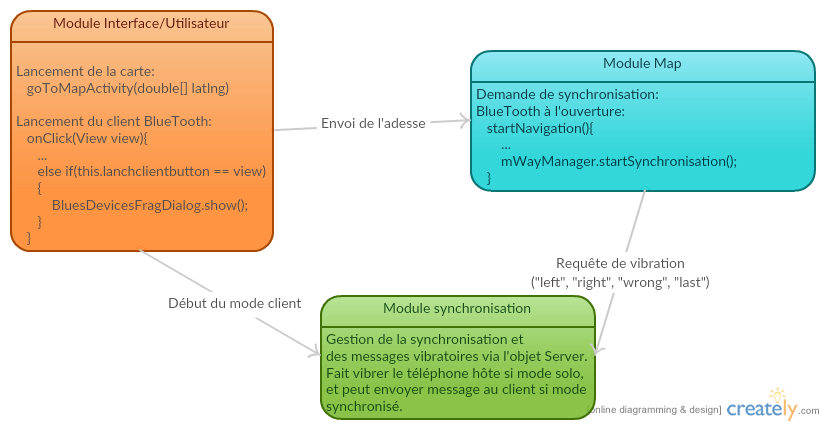
\includegraphics[height=250px]{Assets/Lien_entre_modules.png}
\begin{flushleft}
\hspace*{15pt}\hbox{\scriptsize Source:\thinspace{\scriptsize \itshape \url{http://www.creately.com}}} % Inutile de mettre une source d'un dessin que tu as fait toi-même
\end{flushleft}
\captionof{figure}{Lien entre les modules}
\label{LienModule}
\end{center}
L'application GPS pour les malvoyants est composée de 3 modules : un module "Map" qui manipule les cartes et la navigation, un module "Synchronisation" qui est en charge du protocole de communication \textit{BlueTooth} entre les deux téléphones portables et un module "UI" qui représente l'interface utilisateur (accueil de l'application et saisie d'adresse).

\subsection{Module de saisie d'adresse}
\label{subsec:ModuleUI}
\subsubsection{Description générale}
\begin{center}
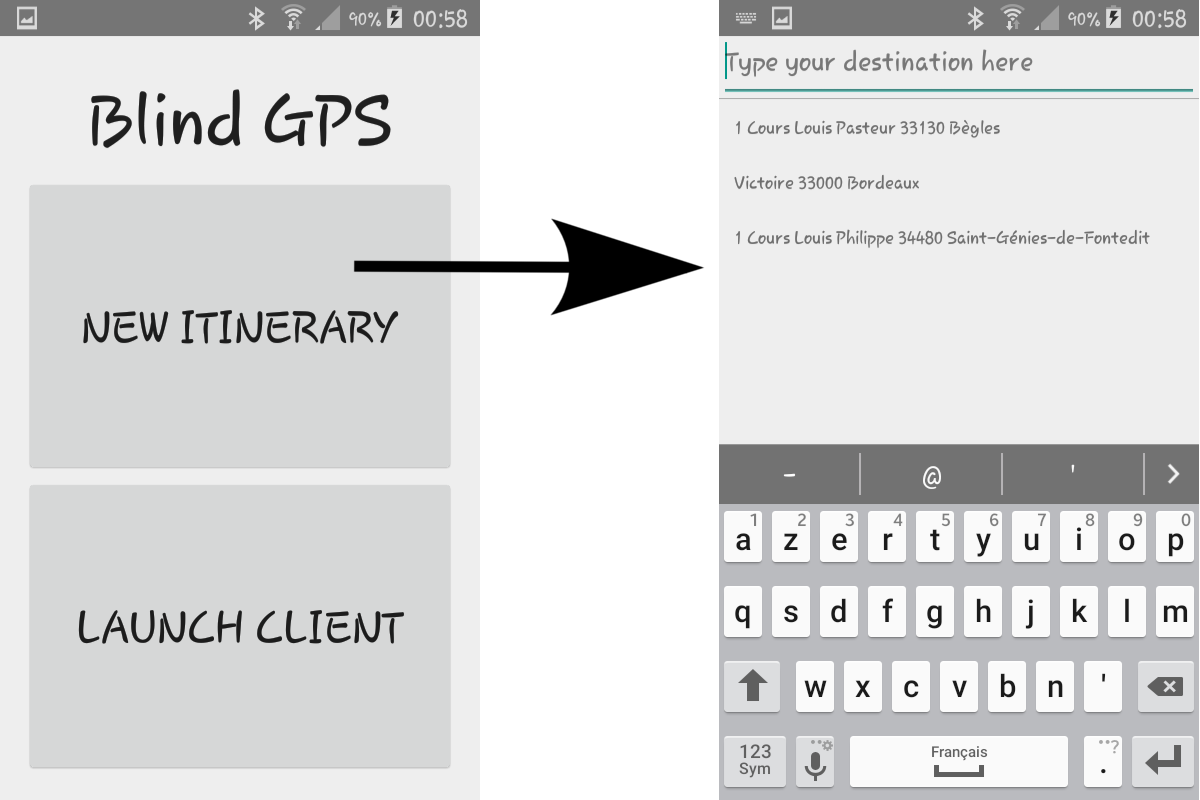
\includegraphics[height=250px]{Assets/screenUI.png}
\captionof{figure}{Capture d'écran de l'ouverture de l'application vers la saisie d'adresse
}
\label{screenUI}
\end{center}
Étant donné que l'application est destinée à un malvoyant, l'interface graphique doit être la plus simple et la plus intuitive possible. Elle est organisée en deux activités, une activité d'accueil et une activité permettant la saisie ou la sélection d'une adresse puis la transition vers le module de navigation. L'activité d'accueil est composée d'un titre, soit le nom de l'application et de deux gros boutons. Le premier bouton permet de démarrer un itinéraire, c'est-à-dire de passer à l'activité de saisie d'adresse, le second bouton permet quant à lui le lancement du couplage \textit{BlueTooth} avec le second appareil. La seconde activité, est composée d'une barre de saisie permettant de saisir l'adresse de destination. A cela s'ajoute en dessous, une liste des dernières destinations utilisées, permettant d'éviter une saisie redondante. De plus, lorsque l'utilisateur entre l'adresse de destination souhaitée, une liste de suggestions vient remplacer la liste des entrées récentes et se met à jour au fur et à mesure que la tape au clavier progresse. Enfin, afin de se différencier d'un GPS classique et de s'adapter au problème de vue de l'utilisateur, une saisie vocale est disponible, et lors de la validation de l'adresse cible, cette dernière est lue par une voix synthétique confirmant l'adresse saisie dans le but de permettre à l'utilisateur de savoir s'il s'est trompé ou non dans l'adresse validée.

\subsubsection{Diagramme des classes}
\begin{center}
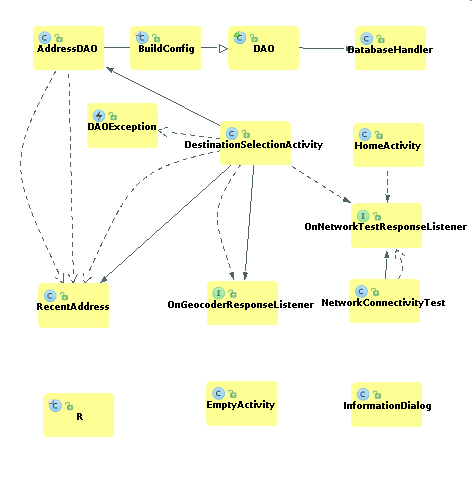
\includegraphics[height=250px]{Assets/uiUML.png}
\captionof{figure}{Diagramme des classes du module UI\\
Flèches à pointe pleine: référence sur, en donnée membre.\\
Flèches à pointe creuse: étend la classe pointée.\\
Flèches pointillées à pointe creuse: implémente la classe pointée.\\
Flèches pointillées à pointe pleine: référence sur, en variable locale à une méthode.}
\label{uiUML}
\end{center}

\subsubsection{Description technique}

\begin{itemize}
\item \textbf{Classe HomeActivity :} lors du lancement de l'application, l'activité "HomeActivity" est affichée (donc ajoutée en haut de la pile des activités). Lorsque l'on clique sur le bouton "New itinerary", la connexion réseau est vérifiée grâce à l'objet "NetworkConnectivityTest" qui vérifie la connectivité réseau. Une fois le test réseau passé, l'activité "DestinationSelectionActivity" est lancé (ajouté au-dessus de l'activité précédente dans la pile des activités). Si le test échoue (application non reliée à Internet), un message d'erreur est affiché indiquant la nécessité d'être connecté à Internet.\\ Pour ce qui est y du clic sur le second bouton, "Launch client", il affiche une boîte de dialogue "BlueDevicesDialogFrag" présente dans le module "Synchronisation" qui permet la sélection de l'appareil \textit{BlueTooth} avec lequel se coupler.\\

\item \textbf{Classe DestinationSelectionActivity :} au lancement de l'activité "DestinationSelectionActivity", un thread est lancé en tâche de fond qui permet d'effectuer des requêtes grâce à l'objet "Geocoder" pour obtenir des suggestions d'adresses. La classe "Geocoder" est une classe native de l'API \textit{Android} permettant la récupération d'adresses postales, et leurs informations associées, dont la longitude et la latitude, utilisées pour la navigation. Ainsi, à chaque nouveau caractère tapé dans la barre d'entrée d'adresse, une requête est soumise au thread "GeocoderDialog" et une requête de suggestions est envoyé. A la réception des nouvelles suggestions, la liste des suggestions est mise à jour via la fonction "onGeocoderResponse()" (\underline{pattern Listener}). Après avoir obtenu aperçu dans la liste des suggestions, l'adresse de destination souhaitée, l'utilisateur sélectionne la suggestion et amorce ainsi la méthode "callback" "onTouch()". En premier lieu, l'adresse sélectionnée est récupérée via un unique identifiant dans la liste. Puis, elle est insérée dans la base de donnée, grâce à l'objet "AddressDAO" et la méthode "insert()". Si elle n'était pas présente dans la base, elle est insérée normalement, si c'était le cas, son compteur d'utilisations et sa date de dernière utilisation (ce qui permet de classer les entrées récentes par date de dernière utilisation) sont simplement mis à jour. Ensuite,l'adresse est lue via l'objet "TextToSpeech", qui permet une synthèse vocale, si la fonctionnalité est supportée par l'appareil. Enfin, la méthode "goToMapActivity()" est lancé et permet la transition vers l'activité de navigation tout en lui passant la longitude et la latitude de l'adresse sélectionnée.\\
L'utilisateur peut aussi être exempté de tape au clavier redondante s'il a déjà tapé cette adresse auparavant. Grâce à la base de données, les entrées récentes sont affichées (classées de la plus récente à la moins récente) et il n'a plus qu'à simplement sélectionner celle désirée. Dans ce cas précis, la date de dernière utilisation et le compteur d'utilisations sont juste mis à jour grâce à la fonction "update()" dans la base de données.\\
{\it \underline{Note d'implémentation :} il est aussi important de souligner que l'utilisation d'un thread en tâche de fond pour les requêtes vers le "Geocoder" permet de soulager le thread UI (thread principal de l'application) de l'attente des réponses et par conséquent de fluidifier la tape au clavier dans le champ d'adresse. Aussi, si on regarde la méthode "callback" "onGeocoderResponse()" :}

\begin{lstlisting}
@Override
public void onGeocoderResponse(final List<Address> addresses) {
    new Handler(getMainLooper()).post(new Runnable() {
        @Override
        public void run() {
            suggestionsListData = addresses;
            displaySuggestions();
        }
    });
}
\end{lstlisting}

{\it on remarque qu'on fait appel à un objet "Handler" qui envoie (méthode "post()") un objet "Runnable" à la boucle principale (le thread qui gère les éléments graphiques entre autres). Tout ceci signifie en fait qu'on indique à la boucle principale d'exécuter la fonction "run()" à la place du thread courant. Car dans un système Android, il y a une contrainte de modification sur les éléments graphiques, seul le "thread UI" (boucle principale) peut modifier ses éléments graphiques. Nous sommes donc obligés de lui faire mettre à jour sa liste de suggestions par lui-même.}\\

\item \textbf{Classe NetworkConnectivityTest :} permet d'effectuer un test de connectivité réseau. Tout d'abord, le statut de l'interface réseau du téléphone est vérifié pour savoir si une connexion (\textit{Wifi} ou réseau mobile) est active. Ensuite, un "ping" de test vers le serveur "google.com" est envoyé pour être sûr d'être bien connecté à Internet. Cette classe étend la classe "AsyncTask" (fonctionnement détaillée dans le module de navigation), ce qui lui permet de lancer une tâche de fond. En effet, pendant toute la durée du "ping", une boîte de dialogue "ProgressDialog" est affichée indiquant à l'utilisateur de patienter (avec un "spinner" d'attente). Une fois, le test effectué (dure en général moins d'une demi-seconde), la boîte de dialogue est révoquée et la fonction "callback" "onNetworkTestResponse()" du "client" du test (le "listener") est appelée, ce qui signifie qu'il doit implémenter l'interface "OnNetworkTestResponseListener" et avoir réécrit le "callback" "onNetworkTestResponse()" qui lui permet d'obtenir la réponse du test de manière asynchrone.\\

\item \textbf{Classe InformationDialog :} représente une boîte de dialogue qui indique que l'application doit être connecté à Internet pour fonctionner. Elle est créée et affichée lorsque le test réseau échoue ou lorsque la requête de suggestion n'aboutit pas (à cause de l'absence de connexion réseau).\\
\end{itemize}

Les deux interfaces suivantes permettent d'implémenter le \underline{pattern "Listener"} et contiennent une méthode "callback" (très utilisée dans le système \textit{Android}) appelée lors d'un événement.\\

\begin{itemize}
\item \textbf{Interface OnGeocoderResponseListener :} permet la récupération des suggestions du "Geocoder". Une classe utilisant le "Geocoder" doit implémenter cette interface et en réécrire la méthode "onGeocoderResponse()" pour traiter les suggestions obtenues. 
\item \textbf{Interface OnNetworkTestResponseListener :} permet la récupération du résultat du test de connectivité réseau. Une classe qui teste la connexion réseau doit implémenter cette interface et en réécrire la méthode "onNetworkTestResponse()" pour obtenir le booléen représentant si oui ou non on est bien connecté à Internet.
\end{itemize} 

\subsubsection{Stockage des données}

Afin de stocker les entrées récentes de l'utilisateur de l'application dans le but de lui faire gagner du temps, une base de donnée SQSLite\footnote{\url{https://www.sqlite.org/}}, qui est implémenté nativement dans le SDK \textit{Android}, a été mise en place. Elle permet l'ajout, la suppression et la mise à jour d'adresses utilisées par l'utilisateur. L'implémentation suit le \underline{pattern "DAO"} ("Data Access Object") dont je me suis fortement inspiré sur le tutoriel d'\textit{OpenClassrooms}\cite{BDD}.

\begin{itemize}
\item \textbf{Classe DatabaseHandler :} cette classe permet la manipulation de la base de données du mobile, elle étend la classe "SQLiteOpenHelper" qui est la classe native qu'il faut étendre pour pouvoir toucher à la base de données. Grâce à l'objet "SQLiteDatabase", on peut y ajouter ou supprimer des tables. La méthode "onCreate()" est appelée à la première utilisation de l'application et la méthode "onUpgrade()" lors d'une mise à jour de l'application (reset des tables).\\
\item \textbf{Classe abstraite DAO :} elle permet la manipulation de la base de données d'un point de vue de l'application, elle gère un objet "DatabaseHandler" et propose des méthodes génériques (ouverture en écriture, ouverture en lecture, fermeture, obtention). Cette classe doit obligatoirement être étendu pour spécifier des méthodes qui manipuleront les tables.\\
\item \textbf{Classe AddressDAO :} comme expliqué précédemment, c'est la classe qui va contenir les méthodes spécifiques à la table "RecentAddresses" et étendre la classe "DAO". Elle manipule l'objet "SQLiteDatabase" (qui représente une base de donnée ouverte en écriture dans ce cas) et utilise les méthodes de cette objet pour modifier la table (insertion, suppression, modification, obtention d'entrées). Si une erreur survient lors d'une manipulation, une exception "DAOException" est levée.\\
\item \textbf{RecentAddress :} structure de données représentant une adresse utilisée par l'utilisateur et sauvegardée dans la base de données. Les suggestions sont représentées par cette objet, ils sont créés lors de la récupération de la liste de suggestions depuis la base de données. Cette structure contient un identifiant unique et un intitulé, qui seront assignés aux "views" graphiques les représentant, un compteur d'utilisations et une date de dernière utilisation. Étant donné que cette structure étend la structure de données native "Address", elle possède aussi une longitude et une latitude qui seront utiles pour la navigation.
\end{itemize}

\newpage
\subsection{Module de gestion de cartes et de navigation}

\subsubsection{Description générale}

\begin{center}
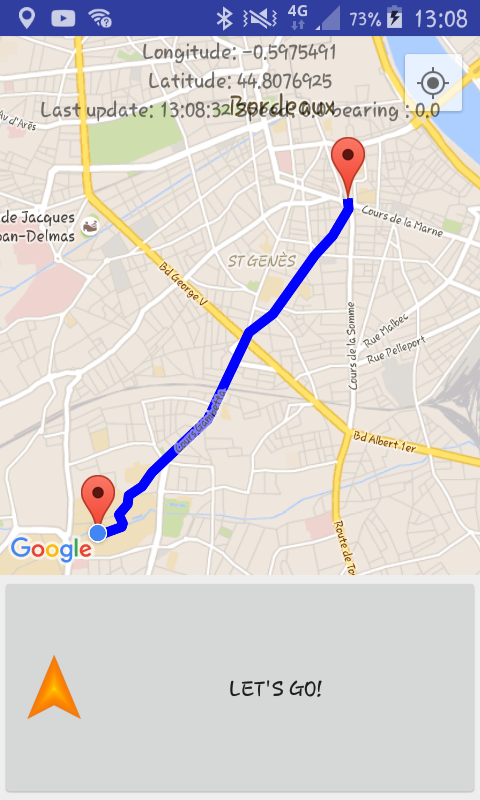
\includegraphics[height=250px]{Assets/screenMap.png}
\captionof{figure}{Capture d'écran de l'écran de carte}
\label{screenMap}
\end{center}

Une fois que l'utilisateur a saisi une adresse, la carte s'affiche et dessine l'itinéraire à partir de la position courante jusqu'à la destination entrée. L'utilisateur a accès à un bouton en haut à droite de l'écran afin de centrer la caméra sur sa position, et un plus gros bouton en bas de l'écran afin de lancer la navigation. Lorsque l'utilisateur clique sur ce bouton, la caméra se place derrière le curseur de position et l'application va maintenant faire vibrer le ou les téléphones.\\
Quand aucun autre téléphone n'est couplé, il est en mode solo, c'est-à-dire qu'il vibrera une fois pour aller à droite et deux fois pour aller à gauche lorsqu'il s'approchera d'une intersection. Lorsque un téléphone se connecte (Voir section \ref{subsec:ModuleUI}),la navigation passe en mode synchronisation, c'est-à-dire que l'utilisateur va pouvoir choisir, au moyen d'une boite de dialogue, quel téléphone sera délégué de vibrer à droite. \\Dans les deux modes, d'autres messages vibratoires lui seront envoyés. Quand l'utilisateur est sur le bon trajet mais qu'il avance dans le sens inverse, des vibrations saccadées lui indiqueront à intervalles réguliers jusqu'à ce qu'il fasse demi-tour. Quand il s'éloigne du chemin, des vibrations saccadées sont aussi transmises mais, différentes de celles du mauvais sens et l'application recalculera un nouvel itinéraire quand il sera trop éloigné. Enfin, une vibration continue lui indiquera quand il sera prêt ou sur le point d'arrivée. 

\newpage
\subsubsection{Diagramme des classes}
\begin{center}
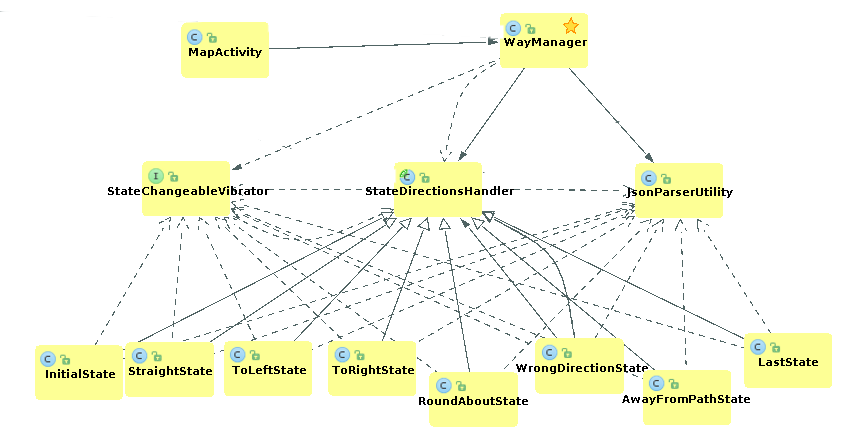
\includegraphics[height=250px]{Assets/mapUML.png}
\captionof{figure}{Diagramme des classes du module Map\\
Flèches à pointe pleine: référence sur, en donnée membre.\\
Flèches à pointe creuse: étend la classe pointée.\\
Flèches pointillées à pointe creuse: implémente la classe pointée.\\
Flèches pointillées à pointe pleine: référence sur, en variable locale à une méthode.}
\label{mapUML}
\end{center}

\subsubsection{Description technique}

Nous allons présenter les différentes classes les plus importantes au fonctionnement de ce module, en passant par l'activité qui contient tout jusqu'aux classes gérant les différents états.
\paragraph{Gestion de la carte et de l'itinéraire}

\begin{lstlisting}
public class MapActivity extends FragmentActivity
        implements OnMapReadyCallback, GoogleApiClient.ConnectionCallbacks, GoogleApiClient.OnConnectionFailedListener, LocationListener 
\end{lstlisting}

Cette classe contient la seule activité du module et implémente les différentes interfaces afin de communiquer avec les services \emph{Google}. En instanciant un objet de classe "GoogleApiClient", qui est le point d'entrée aux services, elle récupère la carte du monde, contient des méthodes "callbacks" de connexions afin de traiter une éventuelle perte de signal et contient aussi les méthodes pour récupérer la position courante. Des fonctions de requêtes d'activation de connexion Internet lui sont aussi déléguées afin de demander à l'utilisateur d'activer sa connexion si celle-ci n'est pas active.

\begin{lstlisting}
public class WayManager extends AsyncTask<Void,Void,Void> implements Parcelable, StateChangeableVibrator
\end{lstlisting}

Cette classe, contenue par "MapActivity", est en charge des comportements de l'application lorsque l'utilisateur est en navigation. Elle est instanciée dès que "MapActivity" est connectée, par la fonction "onConnected()" de l'interface "ConnectionCallBacks". Elle étend la classe "AsyncTask<Params, Progress, Result>" qui est une classe permettant de lancer des actions généralement longues en tâche de fond à l'appel de la méthode "execute()" par trois méthodes à redéfinir:
\begin{itemize}
\item onPreExecute(): méthode appelée sur le thread courant avant que la tâche ne soit exécutée. Elle est en général utilisée pour instancier les données utiles au bon déroulement de la tâche.
\item doInBackground(Params...): méthode qui lance un nouveau thread dès que "onPreExecute()" est terminée et qui exécute son implémentation en tâche de fond.
\item onPreExecute(Result...): méthode directement appelée sur le thread appelant à la fin de la tâche de "doInBackground()".
\end{itemize}
"WayManager" est la classe qui envoie une requête HTML aux services \textit{Google} afin de demander le meilleur itinéraire, et ceci est une action potentiellement très longue. C'est pourquoi il a été choisi de lancer une fenêtre modale dans "onPreExecute()" et de bloquer l'application jusqu'à ce que doInBackground() ait fini de récupérer le fichier JSON qui décrit l'itinéraire, et que "onPostExecute()" ferme la fenêtre modale.\\
C'est aussi la classe qui dessine sur la carte l'itinéraire, qui gère les mouvements de caméra et qui gère le lien avec le module de synchronisation. Pour ce dernier point, elle contient des méthodes pour commencer la synchronisation et la terminer, mais aussi des méthodes d'envoi de messages aux modules. Elle enverra par exemple au module synchronisation l'information "gauche" pour indiquer qu'il doit faire vibrer pour tourner à gauche, selon le mode "solo" ou le mode "synchronisé" que "WayManager" n'a pas besoin de connaître.\\
Elle possède une méthode "event(Location location, boolean onWay)" qui est appelée par "MapActivity" à chaque fois que la localisation change, et qui est en charge de mettre à jour les objets d'états que nous décrirons plus loin.

\begin{lstlisting}
public class JsonParserUtility implements Parcelable
\end{lstlisting}

Cette classe est celle qui récupère et traite l'itinéraire sous format JSON. Elle est codé à l'aide de l'objet "JSONParser" fourni par le kit de développement \textit{Android}. En réalité, c'est les actions de cette classe qui sont exécutées dans l'action en tâche de fond de \textit{WayManager}. Elle récupère le fichier, vérifie son intégrité et permet d'accéder aux champs par des méthodes qui simplifie sa lecture. 

\paragraph{Gestion des états}
Pendant la navigation, l'application doit pouvoir gérer plusieurs états, à savoir: quand l'utilisateur doit tourner à gauche à la prochaine intersection, à droite, quand il est dans le mauvais sens, quand il s'éloigne de la route, quand il s'approche d'un rond-point et quand il s'approche de la ligne d'arrivée. Dans un souci de maintenabilité et de bonne lecture du code, le patron de conception \underline{État} paraît bien adapté à la situation. Une classe abstraite a été implémentée:

\begin{lstlisting}
public abstract class StateDirectionsHandler implements Parcelable
\end{lstlisting}

C'est dans cette classe que l'essentiel des points algorithmiques de navigation sont implémentés.\\Pour une première approche, nous avons développé une fonction permettant de trouver l'angle entre le point courant, la prochaine intersection et celle d'après, en utilisant la \underline{loi des cosinus}. Un angle entre 0 et 120 degrés (valeurs définies statiquement dans cette classe) indiquera que l'utilisateur doit tourner à gauche dans 5 mètre (valeur également définie en tant que constante). Mais, le fichier JSON nous donnant une liste des manœuvres pour chaque point, il nous a paru judicieux de changer d'implémentation et de simplement lire le fichier pour trouver quel est le prochain état. La fonction qui utilisait la \underline{loi des cosinus}, initialement appelée "findNextState(LatLng location)", est finalement renommée "RoundAboutExit(LatLng location)" car elle servira au passage des rond-points. En effet, ceux-ci sont simplement notés dans le fichier JSON "roundabout-right" avec seulement le numéro de la sortie (3th, 1st,...) sans localisation, nous allons donc avoir besoin de cette fonction pour déterminer quand l'utilisateur approche de la sortie.\\
Elle contient aussi des fonctions permettant de traiter les données de localisation pour déterminer si l'utilisateur est dans la mauvaise direction et pour récupérer les points de la ligne dessinée que l'utilisateur doit suivre.

\newpage
\subsection{Module de synchronisation Bluetooth}

\subsubsection{Architecture Client/Serveur}
L'application GPS pour les malvoyants utilise une architecture Client/Serveur. Deux téléphones sont nécessaires pour cela. L'un servira de serveur et le deuxième téléphone sera le client.

Le téléphone serveur sera celui qui affichera la carte, l'itinéraire et la position de l'utilisateur sur la carte. Il est sensé vibrer pour le coté qui lui aura été choisi par l'utilisateur. Par défaut, le téléphone serveur vibre pour le coté droit.

Le téléphone client ne fait qu'exécuter ce que le téléphone serveur lui demande. Il est sensé se connecter au téléphone serveur via la boîte de dialogue qui affichera un ensemble de serveurs éventuels. Ce téléphone vibre pour le coté gauche mais l'utilisateur pourra éventuellement le modifier.

\subsubsection{Protocole de communication}
Le premier téléphone qui se connecte à l'application choisit l'option de démarrer l'application en mode "solo", c'est à dire sans synchronisation. Ce mode permet d'utiliser l'application sans faire appel à un autre téléphone. Dans ce cas, nous utilisons le protocole avec les vibrations mentionné ci-dessus dans la partie des besoins (cf besoins).

Lorsqu'un deuxième téléphone est amené à être utilisé, le deuxième téléphone devra se mettre en mode synchronisation. En sélectionnant ce mode, une boîte de dialogue proposant un ensemble de téléphones auxquels le deuxième téléphone pourra se connecter. Dès lors que les téléphones essayent de se coupler pour la première fois, une boîte de dialogue s'affiche sur les deux téléphones et demandent ainsi l'appareillement. Si l'appareillement a déjà eu lieu une première fois, les fois suivantes, cette boite de dialogue de demande d'appareillement ne s'affichera plus tant qu'ils restent dans la liste des téléphones appareillés pour l'un et pour l'autre.

En cas de déconnexion lors d'une synchronisation, le téléphone délaissé, se mettra directement en mode "solo".
 

\subsubsection{Fiabilité du protocole}
La connexion entre deux téléphones utilisant l'application est entièrement sécurisée. En effet, l'utilisation d'un identifiant unique de connexion (UUID) garantit une connexion qu'entre les téléphones ayant cet identifiant. C'est grâce à cette clé (UUID) que les deux téléphones s'assurent qu'ils se sont connectés dans le cadre de l'utilisation du GPS.
Par cette méthode, seuls les téléphones ayant installés l'application pourront se coupler pour faire usage de l'application.

Le téléphone serveur est apte à détecter une déconnexion du téléphone client qui lui envoie un "ping" toutes les 5 secondes. Lorsque le téléphone serveur ne reçoit plus de "ping", il se passe directement en mode solo car la synchronisation n'est plus établie. Elle peut être relancée par l'utilisateur s'il est à l'origine de cette interruption.

Lorsque le téléphone client détecte l'absence de connexion avec le téléphone serveur car ce dernier ne lui a pas envoyé de "ping" d'acquittement, il se lance en mode solo avec les informations que le téléphone serveur lui aurait communiqué.

\subsubsection{Diagramme des classes}
\begin{center}
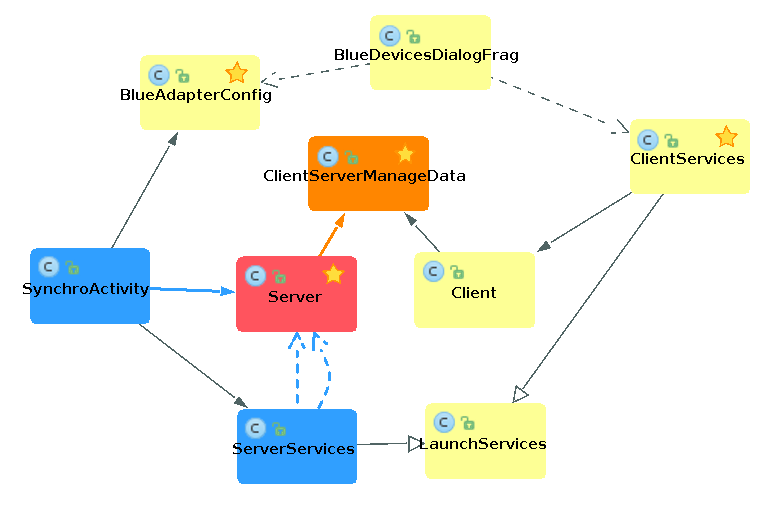
\includegraphics[height=300px]{Assets/synchroUML.png}
\captionof{figure}{Diagrammes de classes du module Synchronisation\\
Flèches à pointe pleine: Référence sur, en donnée membre.\\
Flèches à pointe creuse: Étend la classe pointée.\\
Flèches pointillées: Référence sur, en variable locale à une méthode.}
\label{synchroUML}
\end{center}

\subsubsection{Description technique}

Le module synchronisation gère le cas de l'utilisation de deux téléphones. Il est composé principalement des classes suivantes:

\begin{lstlisting}
public class BlueAdapterConfig implements Parcelable 
\end{lstlisting}

C'est cette classe qui initialise l'adaptateur \textit{Bluetooth}, l'ensemble des appareils auxquels il peut s'appareiller et met en place un ensemble de fonctions comme celle de l'activation du \textit{Bluetooth} avec "enableVisibility()" ou encore celle de recherche des appareils environnants avec "find()".

\begin{lstlisting}
public class BlueDevicesDialogFrag extends DialogFragment
\end{lstlisting}

La classe "BlueDevicesDialogFrag" intervient principalement lorsqu'on lance le mode "synchronisation". Une boîte de dialogue avec l'ensemble des appareils \textit{Bluetooth} visibles. Après sélection de l'appareil serveur dans la liste, le client est créé et la tentative de connexion commence. Une fois le client connecté, un "toast" s'affiche pour indiquer au client que la connexion s'est bien établie.

\begin{lstlisting}
public class Client extends Thread 
\end{lstlisting}

Cette classe sert principalement pour la création d'un nouveau client, c'est à dire un appareil qui tente de se connecter à un autre. Le client envoie toutes les 5 secondes un "ping" au serveur pour que le serveur sache qu'il est toujours connecté ou non.

\begin{center}
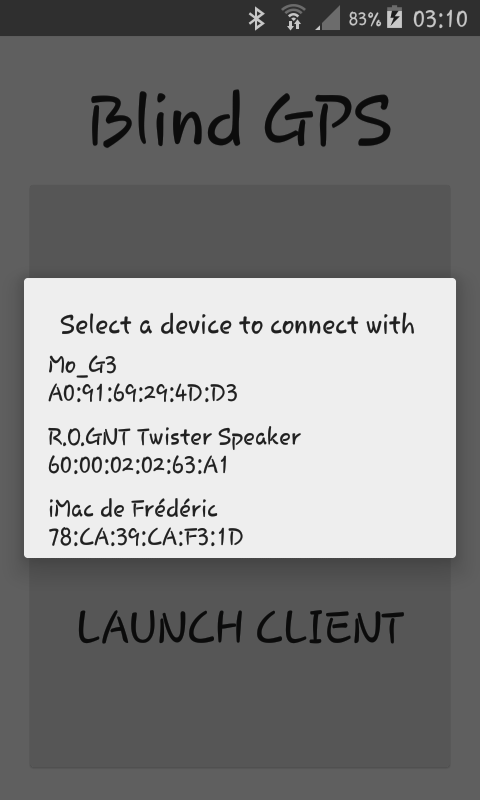
\includegraphics[height=250px]{Assets/client.png}
\captionof{figure}{Capture d'écran de lancement du client}
\end{center}

\begin{lstlisting}
public class Server extends Thread implements Parcelable 
\end{lstlisting} 

Dans cette classe, il est question de la création du serveur, qui représente l'appareil auquel on se connecte. Le serveur accepte la connexion d'un client et lui envoie des messages à travers l'objet "BluetoothSocket". Une fois la connexion établie, le téléphone serveur se voit proposé de choisir s'il veut vibrer pour la gauche ou pour la droite.

\begin{center}
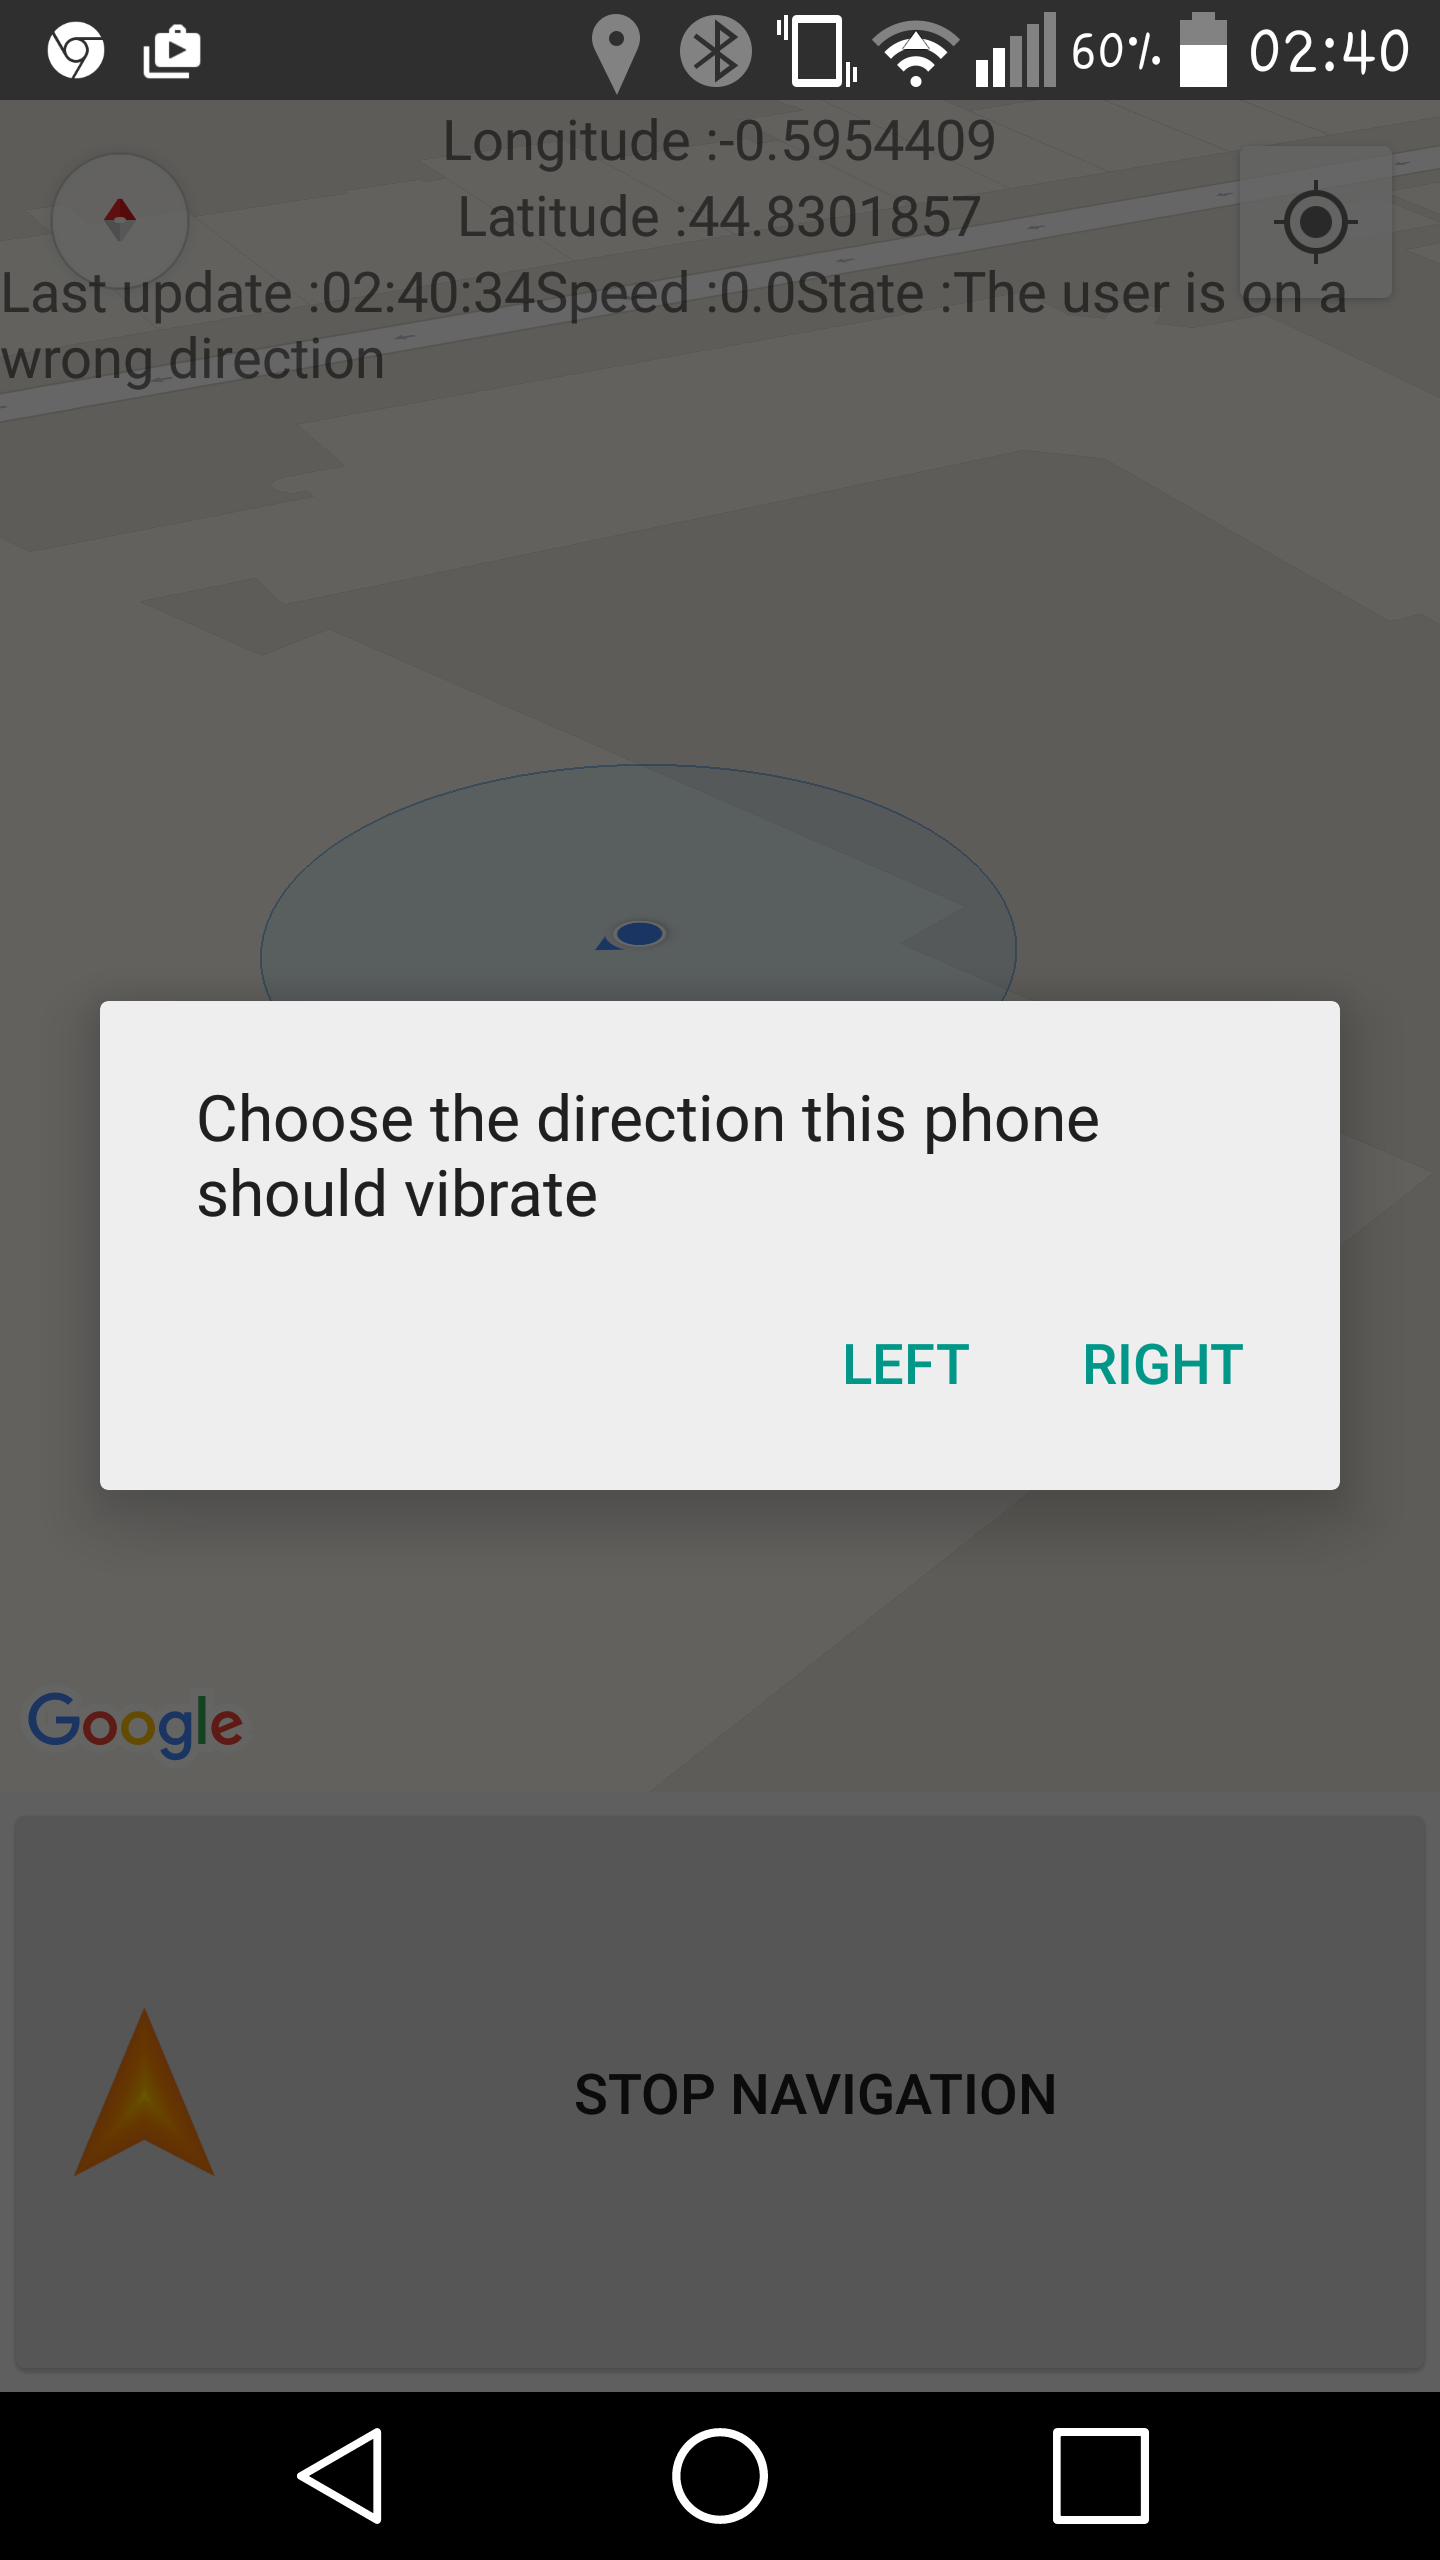
\includegraphics[height=250px]{Assets/Server.png}
\captionof{figure}{Capture d'écran de lancement du serveur}
\end{center}

Après le choix de l'utilisateur, un booléen est mis à jour afin de faire le traitement des messages échangés avec la fonction "writeblue()": 

\begin{lstlisting}
 public void writeBlue(String bytes) {
        if (blueSocket!=null && blueSocket.isConnected()) {
            if((bytes.equals("right") && posRight==true)
            || (bytes.equals("left") && posRight==false))
                vibrator.vibrate(1000);
 [...]
\end{lstlisting} 

\begin{lstlisting}
public class ClientServerManageData extends Thread 
\end{lstlisting}

Dans cette classe, ce sont les traitements des échanges de données entre le client et le serveur qui sont exécutés. Toute donnée entrante ou sortante d'une "socket" passe par cette classe.
Dans cette classe, on détecte aussi la déconnexion d'un client ou d'un serveur grâce aux "pings" ou aux acquittements dans la méthode "run()".

\begin{lstlisting}
[...]
  while (blueInStream.available() < 1) {
                    fin = System.currentTimeMillis();
                    timePing = fin - debut;
                    if (timePing > 9000) {
                        blueInStream.close();
                        blueOutStream.close();
                        blueSocket.close();    
                    }
[...]                    
\end{lstlisting}

Grâce à ce code, il est possible de faire en sorte que le client se mette en mode solo car il n'est plus connecté au serveur.